\section{Cenário de Teste 1}

Este cenário está dividido em 5 (cinco) exemplos, os quais são apresentados a seguir, contemplando todo o processo de auto-localização
em cada exemplo, a partir da apresentação das Imagens abaixo.

\subsection{Exemplo 1}

Exemplo utilizando 200 partículas:

\begin{figure}[H]
  \centering
  \includegraphics[scale=0.4]{figuras/cen1_ex1}
  \caption[Cenário 1 - Exemplo 1]{Cenário 1 - Exemplo 1}
  \label{img:cen1_ex1}
\end{figure}

\subsection{Exemplo 2}

Exemplo utilizando 400 partículas:

\begin{figure}[H]
  \centering
  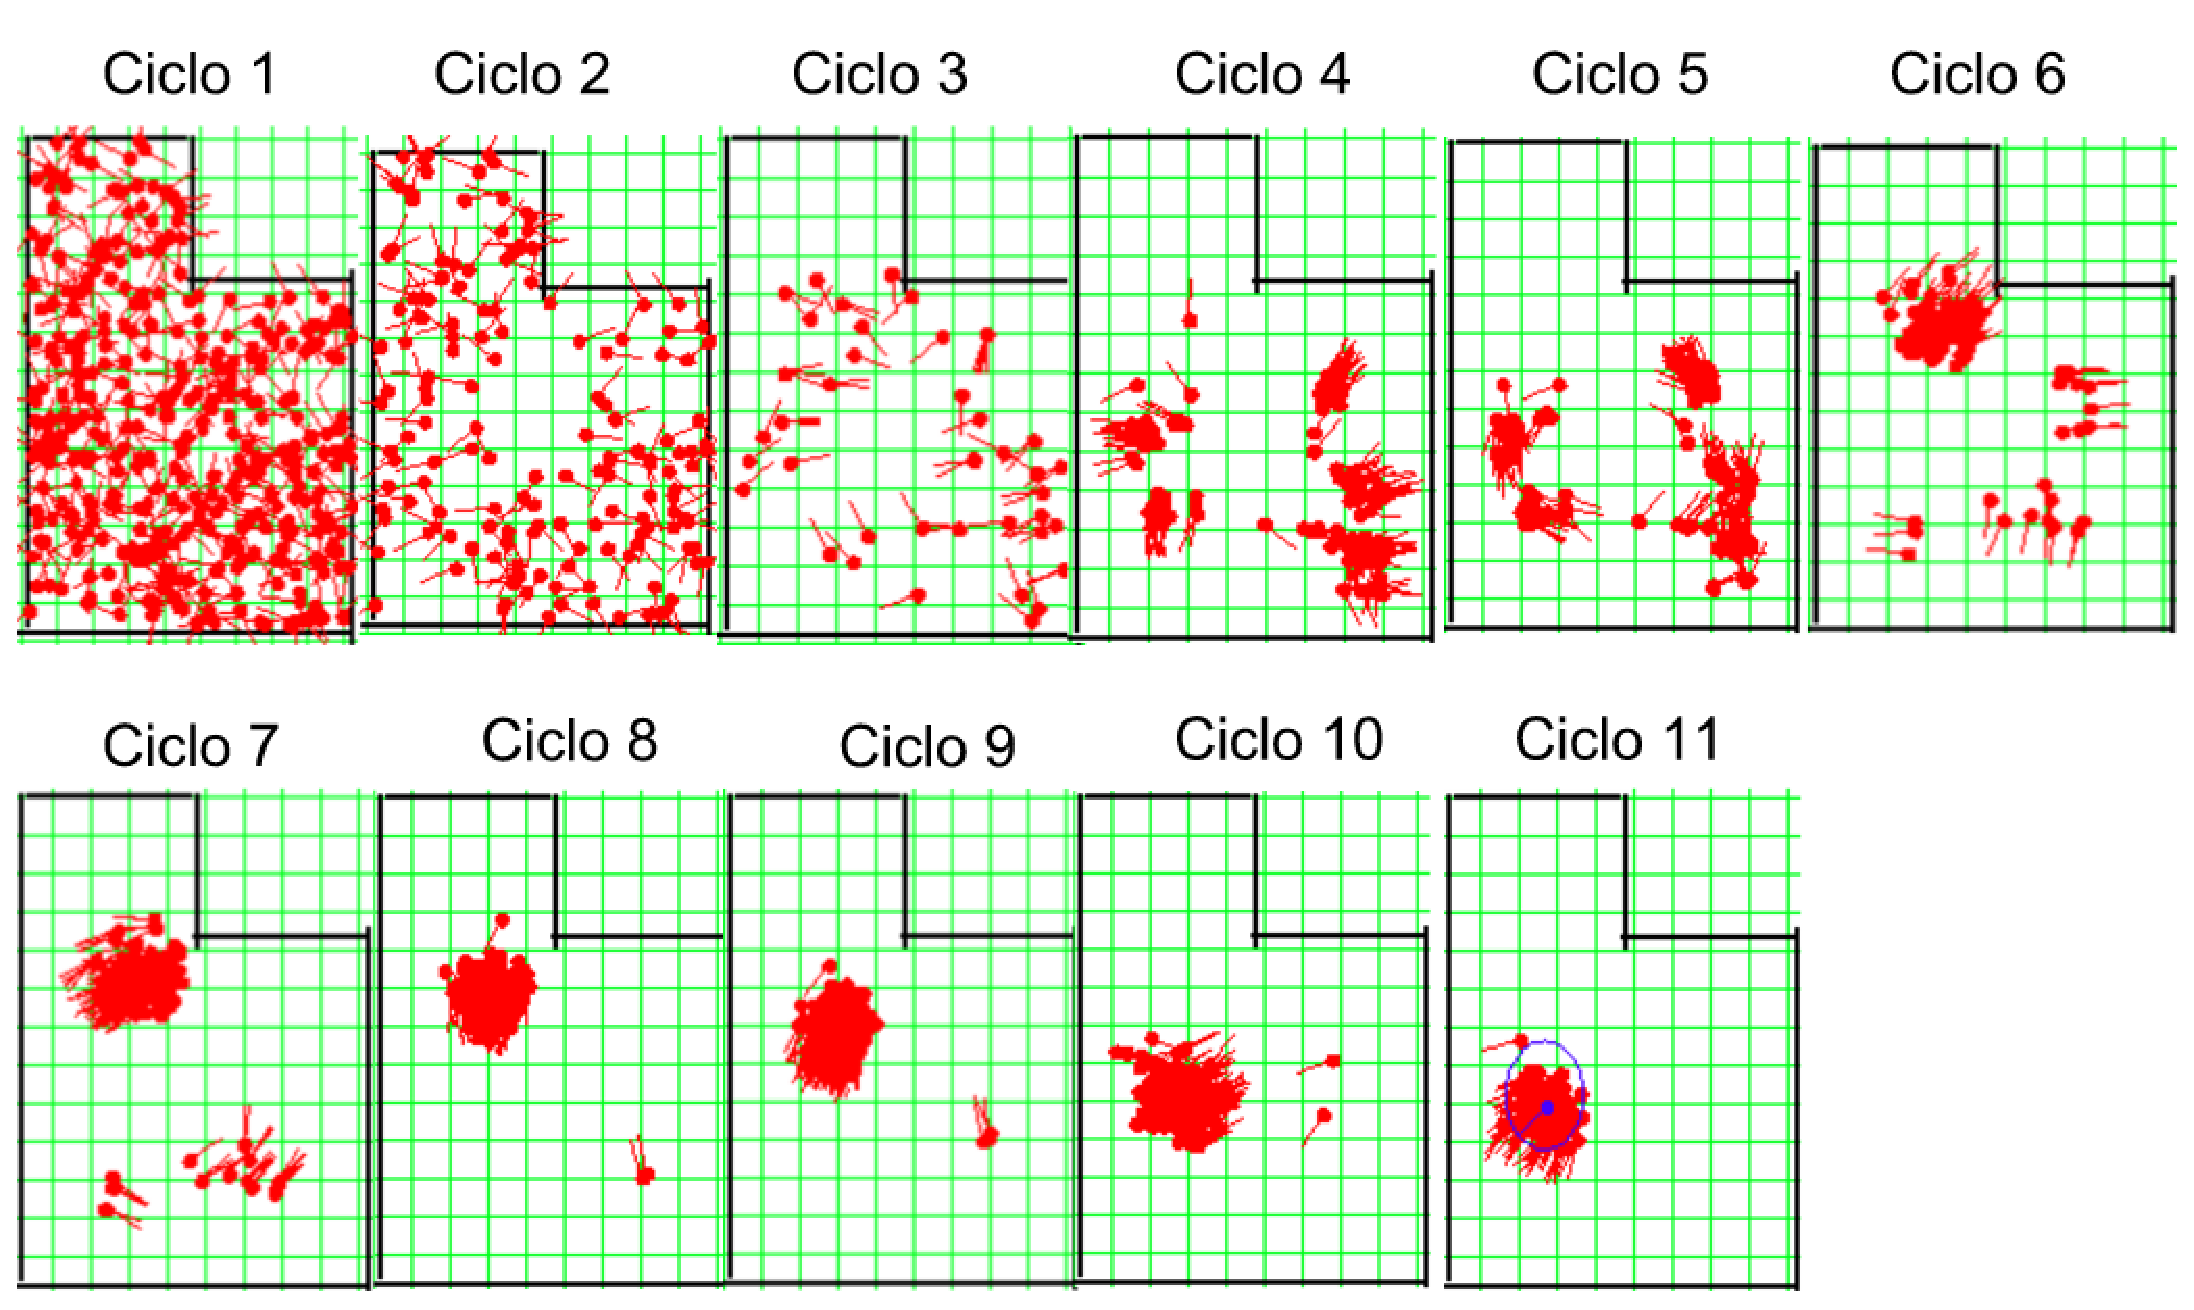
\includegraphics[scale=0.4]{figuras/cen1_ex2}
  \caption[Cenário 1 - Exemplo 2]{Cenário 1 - Exemplo 2}
  \label{img:cen1_ex2}
\end{figure}

\subsection{Exemplo 3}

Exemplo utilizando 500 partículas:

\begin{figure}[H]
  \centering
  \includegraphics[scale=0.4]{figuras/cen1_ex3_1}
  \caption[Cenário 1 - Exemplo 3]{Cenário 1 - Exemplo 3 parte 1}
  \label{img:cen1_ex3_1}
\end{figure}

\begin{figure}[H]
  \centering
  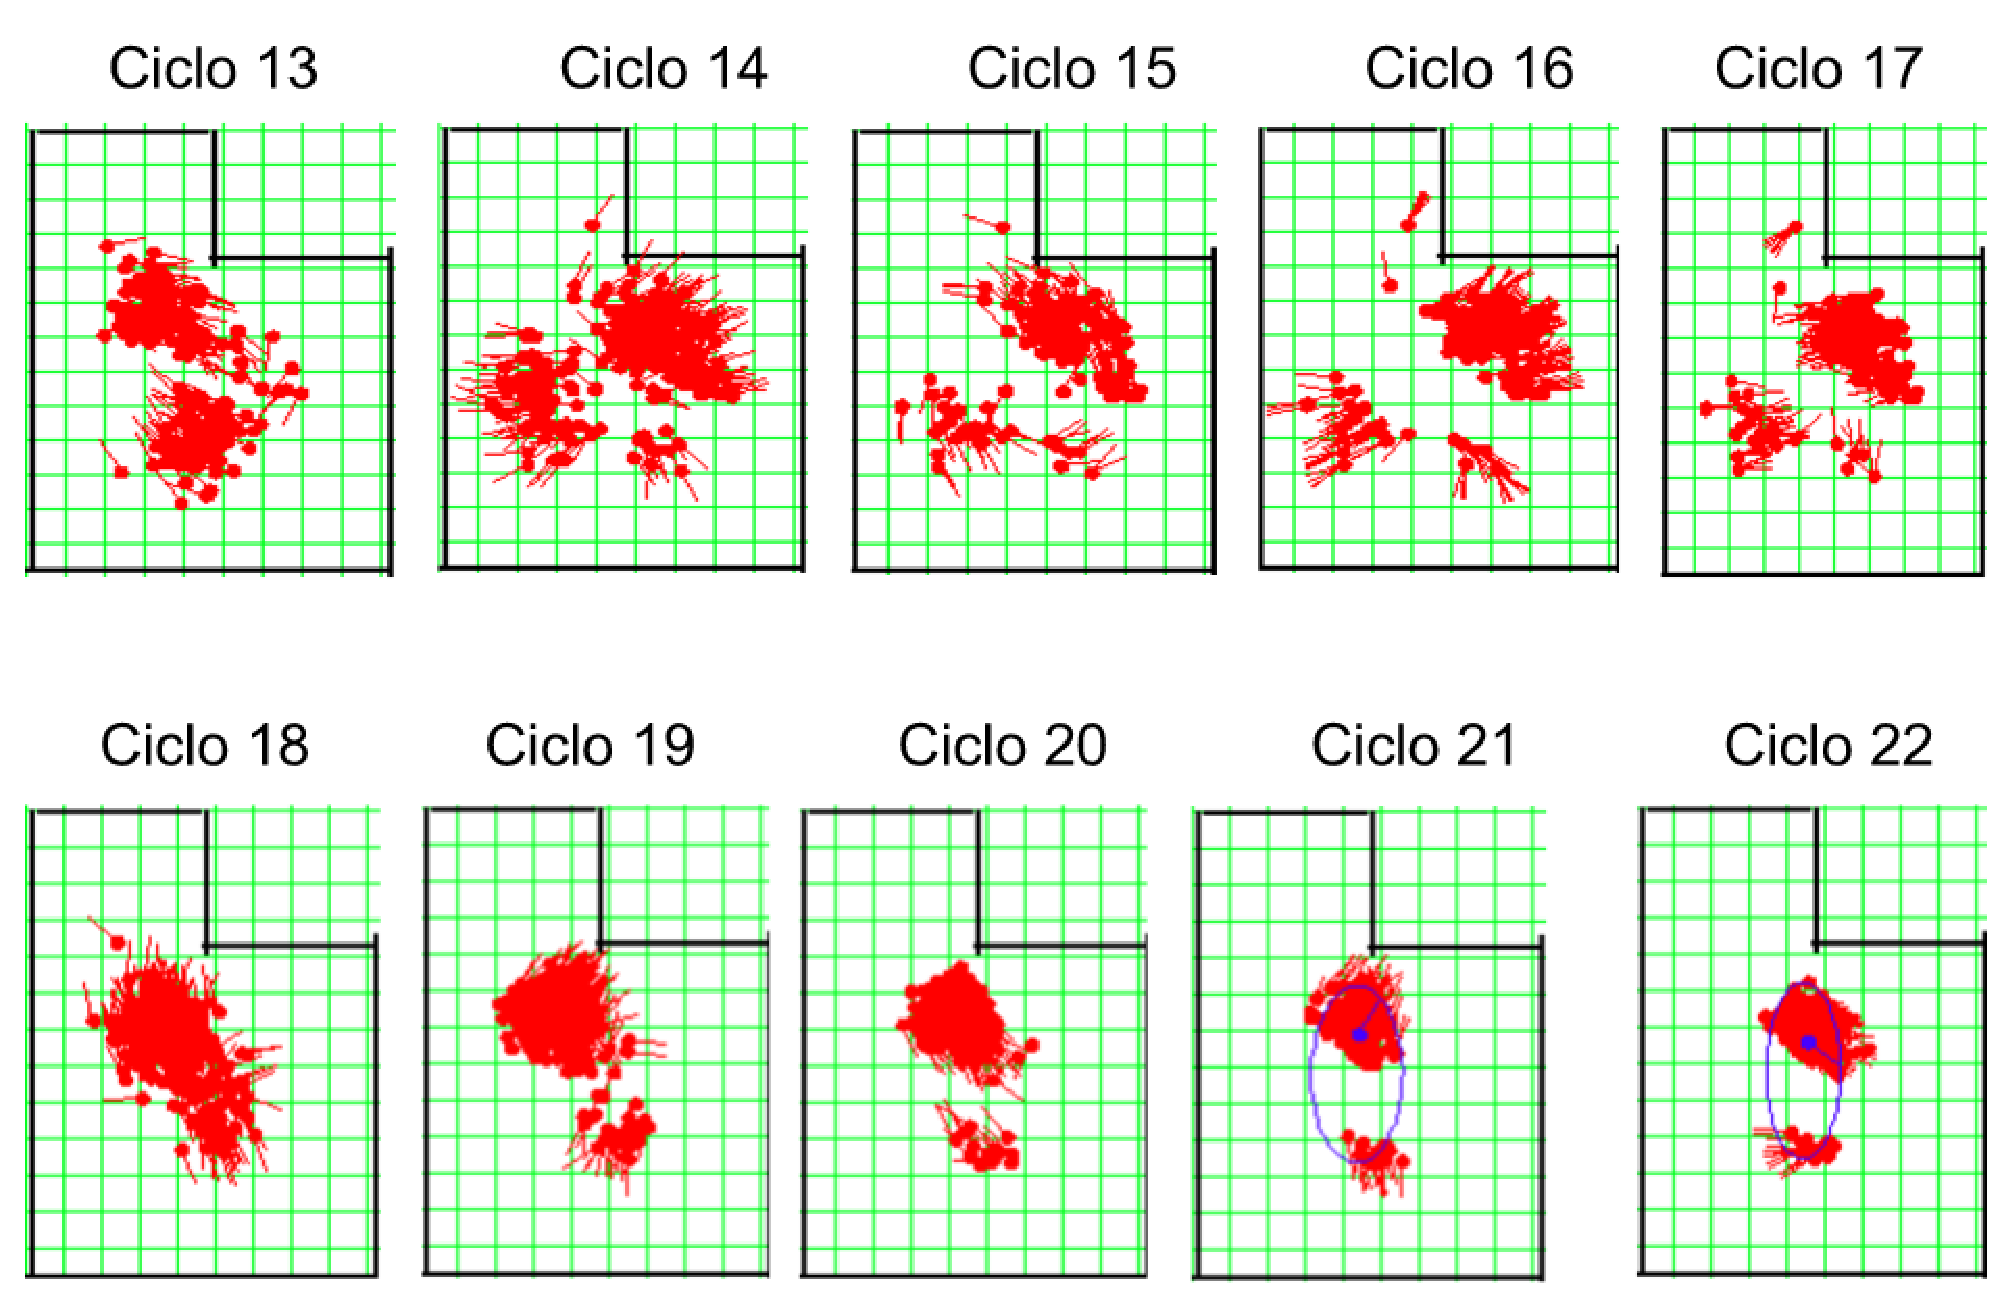
\includegraphics[scale=0.5]{figuras/cen1_ex3_2}
  \caption[Cenário 1 - Exemplo 3]{Cenário 1 - Exemplo 3 parte 2}
  \label{img:cen1_ex3_2}
\end{figure}


\subsection{Exemplo 4}

Exemplo utilizando 100 partículas:

\begin{figure}[H]
  \centering
  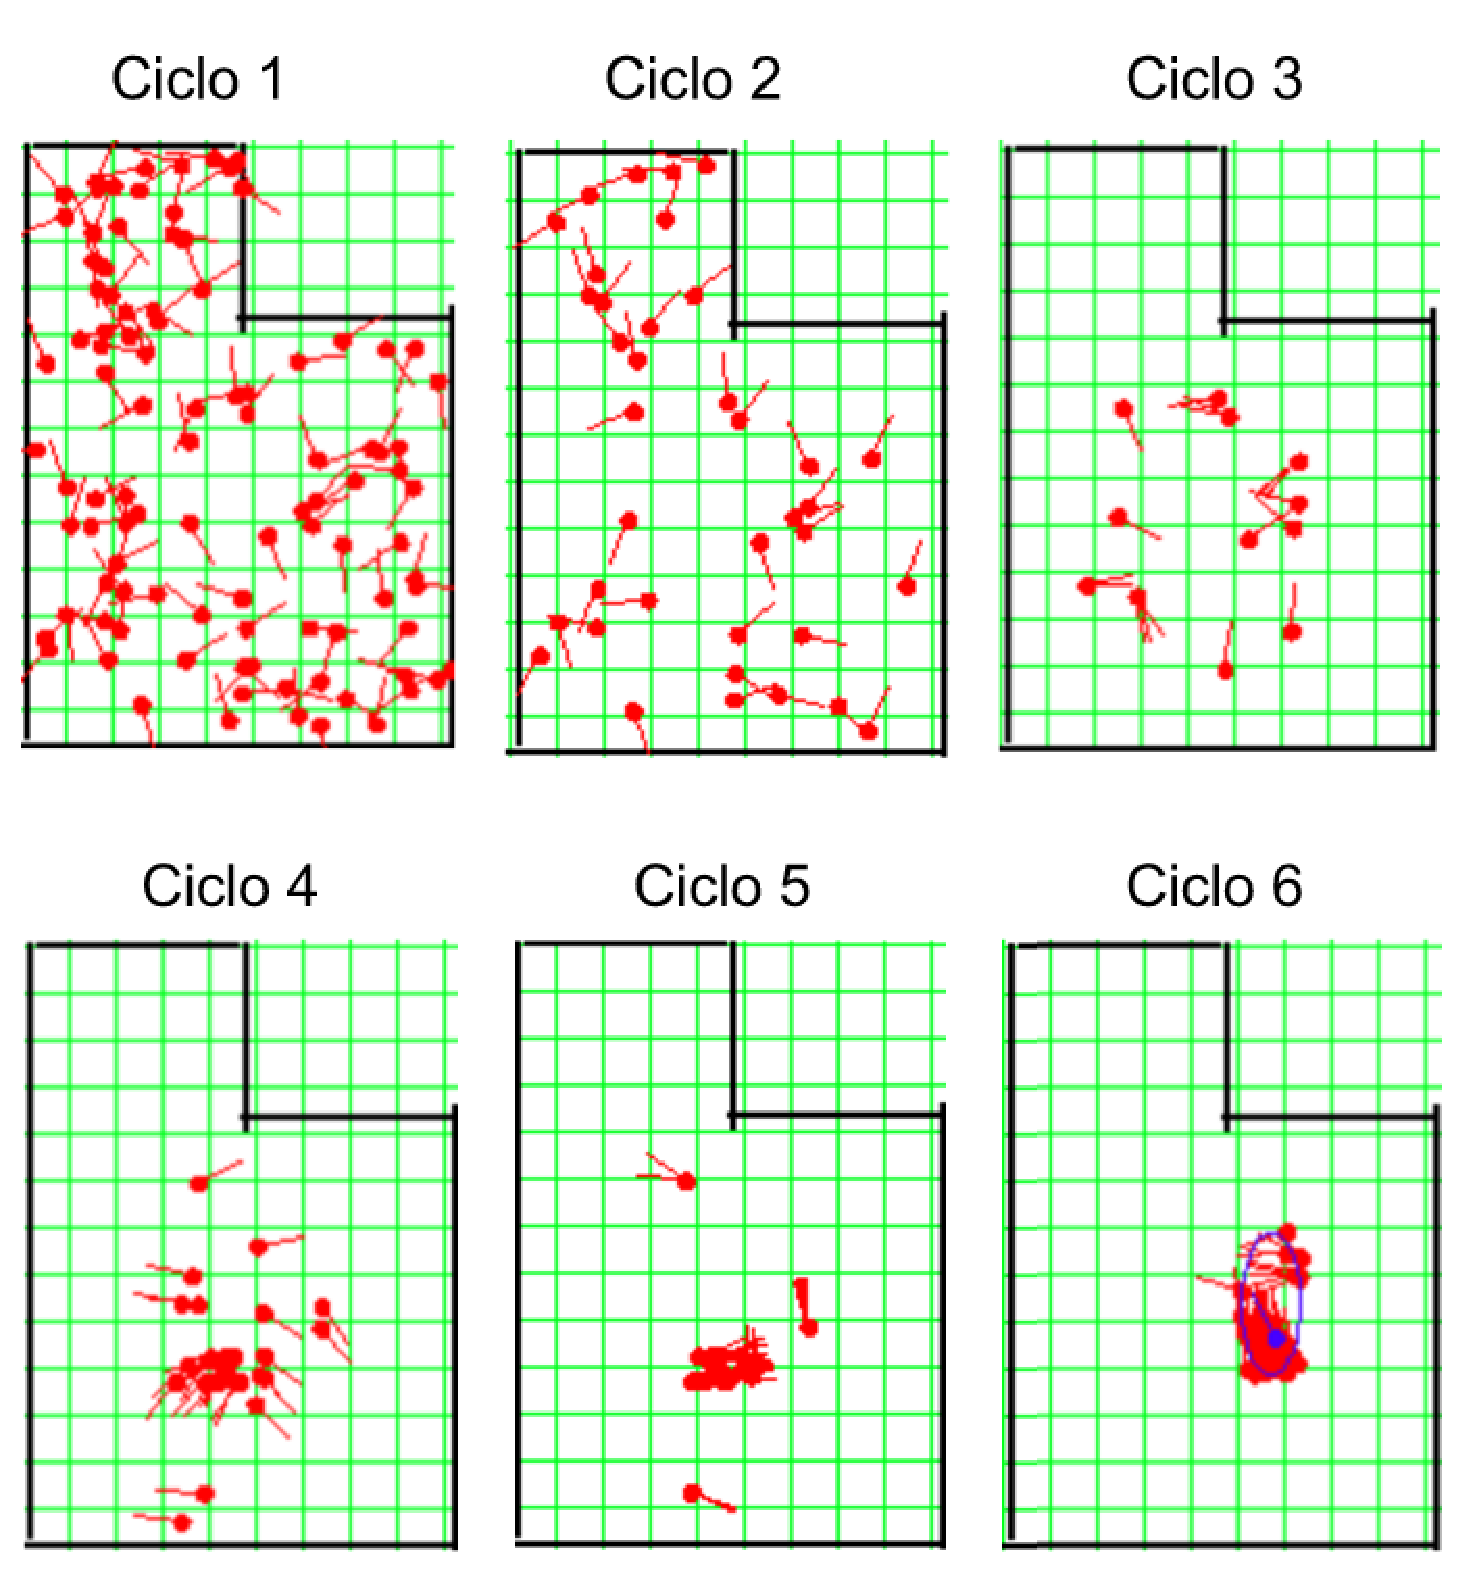
\includegraphics[scale=0.5]{figuras/cen1_ex4}
  \caption[Cenário 1 - Exemplo 4]{Cenário 1 - Exemplo 4}
  \label{img:cen1_ex4}
\end{figure}

\subsection{Exemplo 5}

Exemplo utilizando 150 partículas:

\begin{figure}[H]
  \centering
  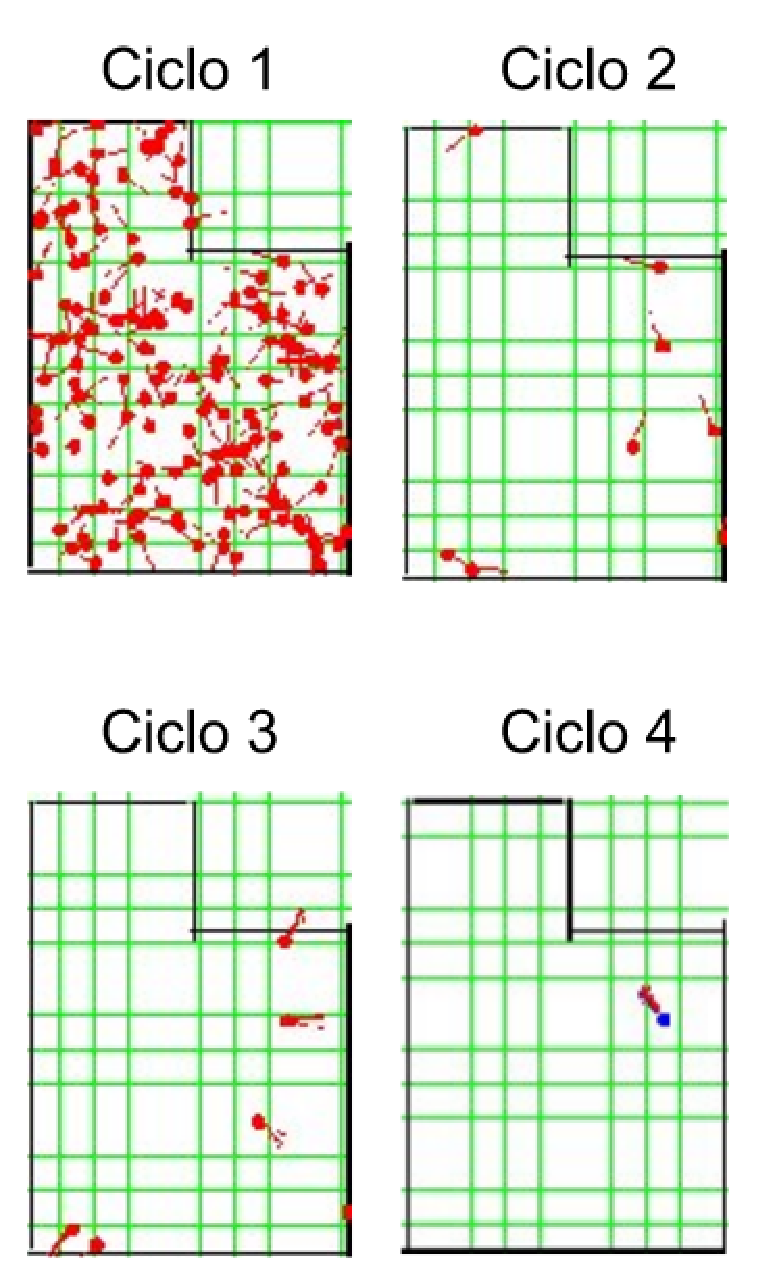
\includegraphics[scale=0.5]{figuras/cen1_ex5}
  \caption[Cenário 1 - Exemplo 5]{Cenário 1 - Exemplo 5}
  \label{img:cen1_ex5}
\end{figure}
